\section{Ricci and the Calculus of Curvature: From Connection to Tensor}

If Christoffel showed us how to differentiate in a curved space,  
then Gregorio Ricci-Curbastro gave us a way to encode that curvature itself—  
not just locally, not just as correction terms, but as a complete algebraic object describing how space bends.

Where Christoffel introduced the symbols \( \Gamma^i_{jk} \) to correct differentiation in a manifold,  
Ricci saw that these corrections could be woven together into something deeper:  
a **tensor calculus** capable of expressing the intrinsic curvature of a space at every point.

\bigskip

\subsection*{The Leap from Christoffel to Ricci}

Christoffel’s symbols were a local tool:  
they told you how to adjust derivatives as you moved along curved coordinates.

But Ricci realized:

✅ The Christoffel symbols themselves were not tensors.  
✅ Their derivatives and products could be combined in a special way to build something **coordinate-independent.**

Ricci constructed the **Riemann curvature tensor** by differentiating Christoffel symbols and combining them with quadratic terms:

\[
R^i_{jkl} = \partial_k \Gamma^i_{jl} - \partial_l \Gamma^i_{jk} + \Gamma^i_{km} \Gamma^m_{jl} - \Gamma^i_{lm} \Gamma^m_{jk}
\]

This object captured **how much space “failed to be flat” when you moved a vector around an infinitesimal loop.**

\bigskip

\begin{tcolorbox}[colback=gray!5!white, colframe=black, title=\textbf{Sidebar: The Shift from Christoffel to Ricci}, fonttitle=\bfseries, arc=1.5mm, boxrule=0.4pt]

\begin{tabular}{>{\raggedright}p{4cm} >{\raggedright}p{5.5cm} >{\raggedright\arraybackslash}p{5.5cm}}
 & \textbf{Christoffel} & \textbf{Ricci} \\
\midrule
Key tool & Christoffel symbols \( \Gamma^i_{jk} \) to correct derivatives & Tensor calculus to encode curvature globally \\
Focus & How to differentiate a vector in curved space & How space itself curves: intrinsic curvature as tensor \\
Equation type & Corrections for derivatives & Riemann curvature tensor; Ricci tensor; full tensor algebra
\end{tabular}

\end{tcolorbox}

\bigskip

\subsection*{From Local Correction to Global Curvature}

Where Christoffel gave us a rule for keeping vectors parallel in a small neighborhood,  
Ricci’s calculus described **the cumulative effect of curvature across a space.**

Ricci’s insight was to build an algebra of tensors:

✅ Objects defined by how they transform under changes of coordinates,  
✅ Objects that preserve intrinsic geometric meaning, even as coordinates shift.

Through this tensor calculus, Ricci encoded the geometric content of Riemann’s vision into a formal system that could be computed, manipulated, and generalized.

\bigskip

In Ricci’s hands, geometry became algebra.

Distances, angles, curvature, and geodesics could all be written as **tensor equations, independent of coordinate choices.**

And as Ricci developed this formalism, he also introduced the **Ricci tensor**—a contraction of the Riemann tensor, summarizing curvature by “summing out” certain directions.

This tensor would soon play a starring role.

\bigskip

\begin{quote}
In Euler, we computed forces.  
In Lagrange, we minimized action.  
In Hamilton, we traced flows.  
In Jacobi, we found surfaces.  
In Cayley, we abstracted transformations.  
In Fourier, we decomposed vibrations.  
In Riemann, we curved the space.  
In Gibbs, we calculated fields.  
In Peano, we defined the space.  
In Christoffel, we corrected differentiation.  
In Ricci, we encoded curvature itself.
\end{quote}

\subsection*{The Language of Curved Spaces Becomes Algebra}

Ricci’s tensor calculus transformed differential geometry into a symbolic system—  
one capable of describing spaces far beyond our physical intuition.

His work wasn’t just a technical improvement over Christoffel’s corrections;  
it was a conceptual leap:  
a shift from local adjustments to a global algebraic structure encapsulating how a space bends in every direction.

But Ricci’s notation and methods were dense, abstract, and ahead of their time.

It would take Tullio Levi-Civita to clarify their geometric meaning.

And it would take Albert Einstein to realize that Ricci’s tensor algebra was nothing less than the mathematical key to gravity itself.

\subsection*{Reinterpreting Kepler’s Second Law Through Ricci’s Tensor Calculus}

Kepler’s Second Law states that a planet sweeps out equal areas in equal times as it orbits the Sun.  
In earlier frameworks, we’ve seen this interpreted as:

\begin{itemize}
    \item A consequence of angular momentum conservation (Gibbs),
    \item A parallel transport condition (Christoffel),
    \item A symmetry of the flow field (Jacobi and Hamilton).
\end{itemize}

But Ricci’s tensor calculus lets us reinterpret this law in a deeper, geometric-algebraic form—  
not as a local conservation law, but as a consequence of the **symmetries in the curvature tensor** itself.

\bigskip

\paragraph{From Symmetry to Conservation.}

In Ricci’s framework, the **geometry of space**—and how it bends—is fully encoded in the Riemann curvature tensor:

\[
R^i_{jkl}
\]

Now consider this:  
Kepler’s Second Law emerges when the **angular momentum is conserved**, and this conservation arises from the **rotational symmetry** of the gravitational field.

But Ricci’s curvature formalism tells us:

\begin{quote}
Every continuous symmetry of the metric corresponds to a Killing vector field,  
and every Killing vector implies a conserved quantity along geodesics.
\end{quote}

In other words:

✅ Kepler’s Second Law is the **observable consequence** of the fact that the spacetime curvature is invariant under rotation.

That rotational symmetry appears in the metric \( g_{ij} \), and is reflected algebraically in the vanishing of the Lie derivative:

\[
\mathcal{L}_\xi g_{ij} = 0
\quad \text{for some Killing vector field } \xi^i
\]

\bigskip

\paragraph{Ricci’s Tensor as the Enforcer of Symmetry.}

In Ricci’s calculus, the presence of a Killing vector leads to the conservation of a momentum-like quantity along a geodesic:

\[
\frac{d}{d\tau} \left( g_{ij} \xi^i \frac{dx^j}{d\tau} \right) = 0
\]

This is the general relativistic version of angular momentum conservation.

So: Kepler’s equal-area sweep isn’t just a quirk of Newtonian motion.  
It’s the projection of a **deeper geometric symmetry**—a conserved quantity arising from the structure of spacetime curvature itself.

\bigskip

\begin{tcolorbox}[colback=blue!5!white, colframe=blue!80!black, title=\textbf{Ricci’s Take on Kepler}]
Kepler measured area.  
Ricci measured symmetry.  
And the Second Law is what happens when the curvature respects rotation.
\end{tcolorbox}


\begin{figure}[H]
    \centering
    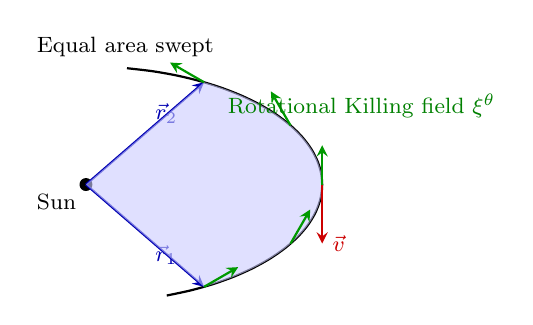
\begin{tikzpicture}[scale=2.5, >=stealth]
    
    % Central mass
    \filldraw[black] (0,0) circle (0.03) node[below left] {\footnotesize Sun};
    
    % Orbit (elliptical-like curve)
    \draw[thick, domain=-70:80, smooth, variable=\t] 
      plot ({1.2*cos(\t)}, {0.6*sin(\t)});
    
    % Two radial vectors at different times
    \draw[->, thick, blue!70!black] (0,0) -- ({1.2*cos(-60)}, {0.6*sin(-60)}) node[midway, below right] {\footnotesize $\vec{r}_1$};
    \draw[->, thick, blue!70!black] (0,0) -- ({1.2*cos(60)}, {0.6*sin(60)}) node[midway, above right] {\footnotesize $\vec{r}_2$};
    
    % Swept area (triangle sectors)
    \fill[blue!20, opacity=0.6] (0,0) -- ({1.2*cos(-60)}, {0.6*sin(-60)}) arc[start angle=-60, end angle=60, x radius=1.2, y radius=0.6] -- cycle;
    
    % Tangent vector at one point (orbital velocity)
    \draw[->, thick, red!80!black] ({1.2*cos(0)}, {0.6*sin(0)}) -- ++(0,-0.3) node[right] {\footnotesize $\vec{v}$};
    
    % Killing vector field (circular)
    \foreach \angle in {-60,-30,0,30,60} {
      \draw[->, thick, green!60!black] 
        ({1.2*cos(\angle)}, {0.6*sin(\angle)}) 
        -- ++({-0.2*sin(\angle)}, {0.2*cos(\angle)});
    }
    
    % Labels
    \node[green!50!black] at (1.4,0.4) {\footnotesize Rotational Killing field $\xi^\theta$};
    \node at (0.2,0.7) {\footnotesize Equal area swept};
    
    \end{tikzpicture}
    \caption{Rotational symmetry as a Killing vector field: The equal-area sweep in Kepler’s Second Law corresponds to a conserved quantity associated with the rotational symmetry of the curved space, encoded via the metric tensor.}
\end{figure}

